\documentclass[12pt]{article}
\usepackage{amsfonts, amssymb, amsmath, amsthm}
\usepackage[margin=1in]{geometry}
\usepackage{tikz}

\title{Explainer: Problem 5 (Rudin 7.13) --- Helly's Selection Theorem}
\author{}
\date{}

\begin{document}
\maketitle

\section*{What's going on?}
We have a sequence of functions $f_n : \mathbb{R} \to [0,1]$, each monotonically increasing. From this sequence, we want to extract a subsequence $f_{n_k}$ that converges \emph{pointwise everywhere}. Part (b) upgrades to uniform convergence on compact sets if the limit is continuous.

This is an ``infinite-dimensional'' version of Bolzano--Weierstrass.

\section*{The big picture: a diagonal argument}

\begin{center}
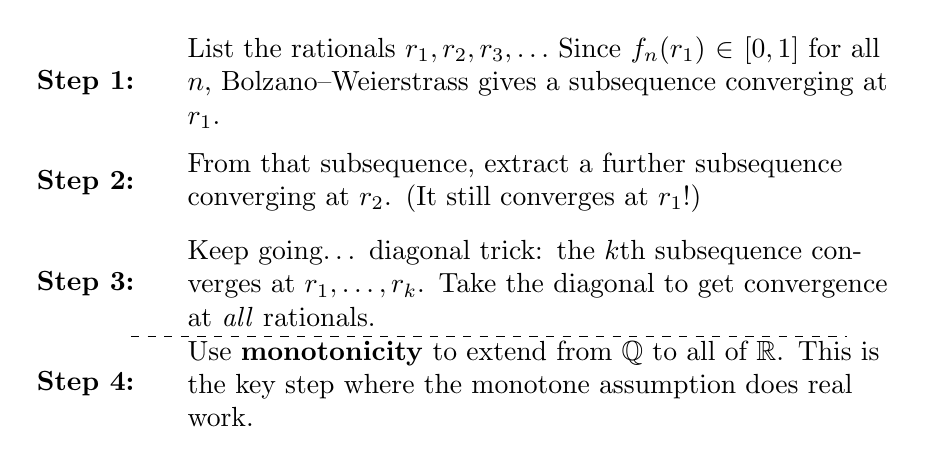
\begin{tikzpicture}[>=stealth, scale=0.85]
    % Rationals
    \node[left] at (-0.5, 3) {\textbf{Step 1:}};
    \node[right, text width=9cm] at (0, 3) {List the rationals $r_1, r_2, r_3, \ldots$ Since $f_n(r_1) \in [0,1]$ for all $n$, Bolzano--Weierstrass gives a subsequence converging at $r_1$.};

    \node[left] at (-0.5, 1.5) {\textbf{Step 2:}};
    \node[right, text width=9cm] at (0, 1.5) {From that subsequence, extract a further subsequence converging at $r_2$. (It still converges at $r_1$!)};

    \node[left] at (-0.5, 0) {\textbf{Step 3:}};
    \node[right, text width=9cm] at (0, 0) {Keep going\ldots\ diagonal trick: the $k$th subsequence converges at $r_1, \ldots, r_k$. Take the diagonal to get convergence at \emph{all} rationals.};

    \draw[dashed] (-0.7, -0.8) -- (10, -0.8);

    \node[left] at (-0.5, -1.5) {\textbf{Step 4:}};
    \node[right, text width=9cm] at (0, -1.5) {Use \textbf{monotonicity} to extend from $\mathbb{Q}$ to all of $\mathbb{R}$. This is the key step where the monotone assumption does real work.};
\end{tikzpicture}
\end{center}

\section*{Why monotonicity matters for Step 4}

Suppose we know $f_{n_k}(r) \to g(r)$ for all rationals $r$. Define $f(x) = \sup\{g(r) : r \leq x, r \in \mathbb{Q}\}$.

At a point $x$ where $f$ is \textbf{continuous}: for any $\varepsilon > 0$, pick rationals $r < x < s$ with $f(s) - f(r) < \varepsilon$. Then
$$
f(r) \leq f_{n_k}(r) + \varepsilon_k \leq f_{n_k}(x) \leq f_{n_k}(s) \leq f(s) + \varepsilon_k
$$
(using monotonicity of $f_{n_k}$), and squeezing gives $f_{n_k}(x) \to f(x)$.

\begin{center}
\begin{tikzpicture}[scale=1]
    \draw[->] (0,0) -- (6,0) node[right] {$x$};
    \draw[->] (0,0) -- (0,3.5) node[above] {};
    \draw[thick, blue, domain=0:5.5, samples=100] plot (\x, {2.5*(1 - exp(-0.7*\x))});
    \node[blue, right] at (5.5, 2.3) {$f$};
    \draw[dashed] (2,0) -- (2, {2.5*(1-exp(-1.4))}) node[above] {};
    \draw[dashed] (3.5,0) -- (3.5, {2.5*(1-exp(-2.45))}) node[above] {};
    \node[below] at (2,0) {$r$};
    \node[below] at (2.75,0) {$x$};
    \node[below] at (3.5,0) {$s$};
    \draw[red, thick, <->] (5, {2.5*(1-exp(-1.4))}) -- (5, {2.5*(1-exp(-2.45))});
    \node[red, right] at (5, {0.5*(2.5*(1-exp(-1.4)) + 2.5*(1-exp(-2.45)))}) {\small $< \varepsilon$};
    \fill (2.75, 0) circle (2pt);
\end{tikzpicture}
\end{center}

Because $f_{n_k}$ is increasing, knowing its values at rationals on both sides of $x$ \textbf{traps} $f_{n_k}(x)$ in a small interval. Without monotonicity, knowing $f_{n_k}$ at rationals tells you nothing about nearby irrationals.

\section*{Dealing with discontinuities of $f$}

The limit $f$ might be discontinuous (monotone functions can have at most countably many jumps). At jump points, the ``squeeze from rationals'' argument fails because $f(r)$ and $f(s)$ don't get close.

But there are only countably many jumps! So apply Bolzano--Weierstrass one more time: from the subsequence that converges at all continuity points, extract a further subsequence converging at all (countably many) discontinuity points.

\section*{Part (b): upgrading to uniform convergence}

If $f$ is continuous, there are \textbf{no} discontinuities to worry about, and the squeeze argument works at every point. On a compact set $[a,b]$, the continuity is uniform, so the squeezing can be made uniform $\Rightarrow$ uniform convergence on $[a,b]$.

\section*{Proof outline}
\begin{enumerate}
    \item Enumerate rationals, use diagonal argument to get subsequence converging on $\mathbb{Q}$.
    \item Define $f(x) = \sup\{g(r) : r \in \mathbb{Q}, r \leq x\}$.
    \item Monotonicity $\Rightarrow$ convergence at all continuity points of $f$.
    \item Extract further subsequence for (countably many) discontinuity points.
    \item For (b): if $f$ continuous, the squeeze is uniform on compact sets.
\end{enumerate}

\end{document}